\documentclass[12pt]{book}

%These tell TeX which packages to use.
\usepackage{array,epsfig}
\usepackage{amsmath}
\usepackage{amsfonts}
\usepackage{amssymb}
\usepackage{amsxtra}
\usepackage{amsthm}
\usepackage{mathrsfs}
\usepackage{color}
\usepackage{eurosym}
\usepackage{times}
%Here I define some theorem styles and shortcut commands for symbols I use often
\theoremstyle{definition}
\newtheorem{defn}{Definition}
\newtheorem{thm}{Theorem}
\newtheorem{cor}{Corollary}
\newtheorem*{rmk}{Remark}
\newtheorem{lem}{Lemma}
\newtheorem*{joke}{Joke}
\newtheorem{ex}{Example}
\newtheorem*{soln}{Solution}
\newtheorem{prop}{Proposition}

\newcommand{\lra}{\longrightarrow}
\newcommand{\ra}{\rightarrow}
\newcommand{\surj}{\twoheadrightarrow}
\newcommand{\graph}{\mathrm{graph}}
\newcommand{\bb}[1]{\mathbb{#1}}
\newcommand{\Z}{\bb{Z}}
\newcommand{\Q}{\bb{Q}}
\newcommand{\R}{\bb{R}}
\newcommand{\C}{\bb{C}}
\newcommand{\N}{\bb{N}}
\newcommand{\M}{\mathbf{M}}
\newcommand{\m}{\mathbf{m}}
\newcommand{\MM}{\mathscr{M}}
\newcommand{\HH}{\mathscr{H}}
\newcommand{\Om}{\Omega}
\newcommand{\Ho}{\in\HH(\Om)}
\newcommand{\bd}{\partial}
\newcommand{\del}{\partial}
\newcommand{\bardel}{\overline\partial}
\newcommand{\textdf}[1]{\textbf{\textsf{#1}}\index{#1}}
\newcommand{\img}{\mathrm{omega}}
\newcommand{\ip}[2]{\left\langle{#1},{#2}\right\rangle}
\newcommand{\inter}[1]{\mathrm{int}{#1}}
\newcommand{\exter}[1]{\mathrm{ext}{#1}}
\newcommand{\cl}[1]{\mathrm{cl}{#1}}
\newcommand{\ds}{\displaystyle}
\newcommand{\vol}{\mathrm{vol}}
\newcommand{\cnt}{\mathrm{ct}}
\newcommand{\osc}{\mathrm{osc}}
\newcommand{\LL}{\mathbf{L}}
\newcommand{\UU}{\mathbf{U}}
\newcommand{\support}{\mathrm{support}}
\newcommand{\AND}{\;\wedge\;}
\newcommand{\OR}{\;\vee\;}
\newcommand{\Oset}{\varnothing}
\newcommand{\st}{\ni}
\newcommand{\wh}{\widehat}

%Pagination stuff.
\setlength{\topmargin}{-.3 in}
\setlength{\oddsidemargin}{0in}
\setlength{\evensidemargin}{0in}
\setlength{\textheight}{9.in}
\setlength{\textwidth}{6.5in}
\pagestyle{empty}

\begin{document}

\begin{center}
{\Large DATA 221 \\  Homework 5  (rev 0)}\\
\textbf{W. Trimble}\\ %You should put your name here
Due: Friday 2022-05-06  - 11:59pm
\end{center}

\vspace{0.2 cm}



\begin{enumerate}

\item
Use a logistic regression model to fit the UCI Credit Default dataset.  You should standardize the inputs and prepare a testing set separate from the training set.
Report the column names and coefficients ordered by the absolute value of the regression coefficient.
% 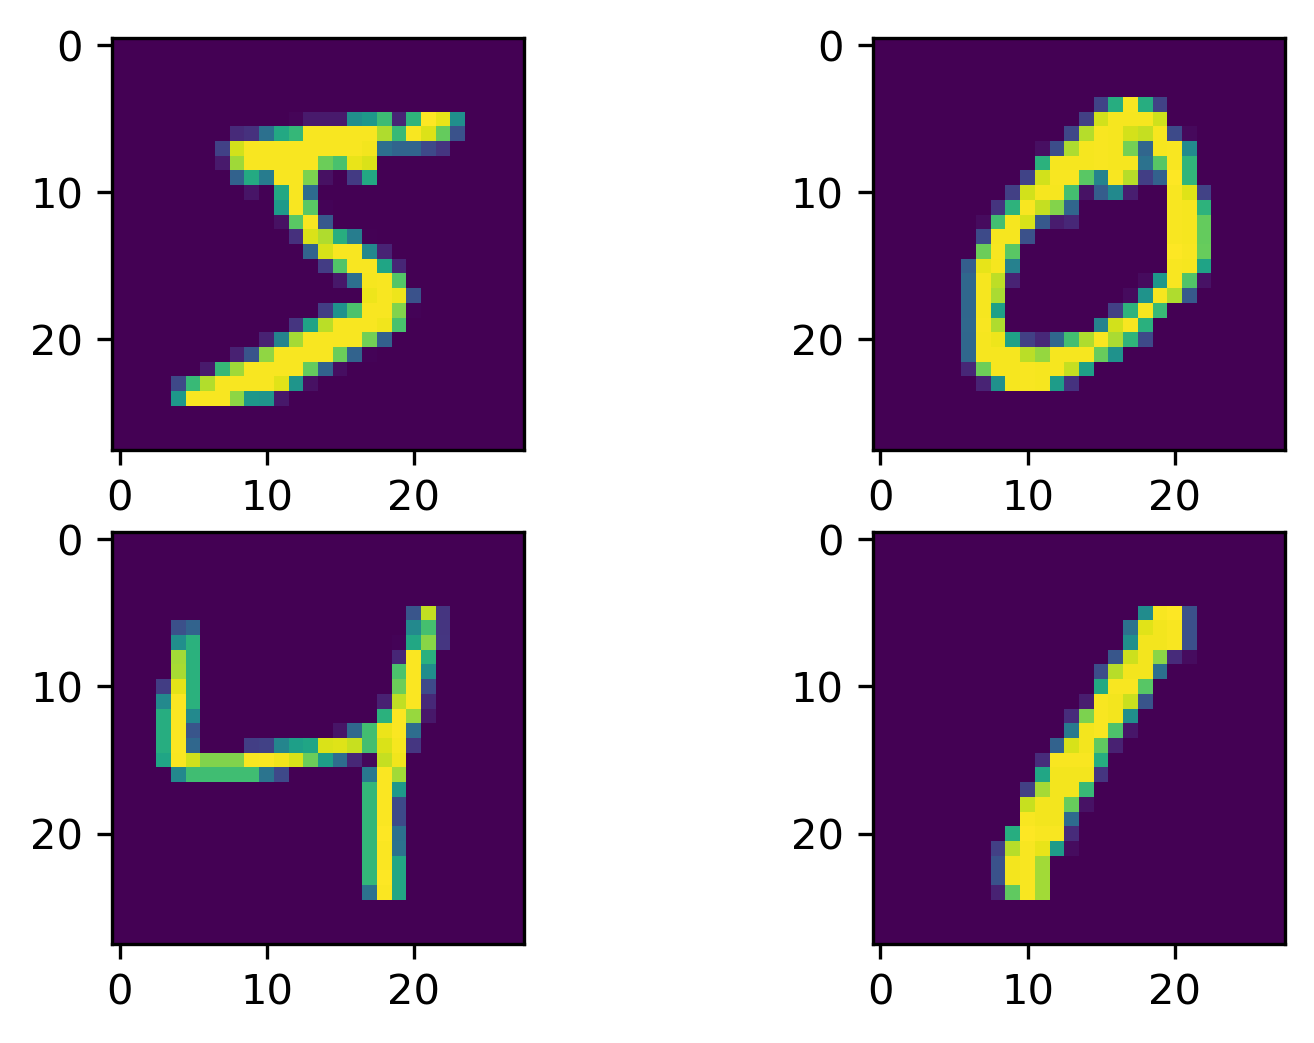
\includegraphics[width=3in]{MNIST.png}

\item
Regularization 

Find the logistic regression coefficients for this dataset with L1 regularization.  
Plot the regression coefficients as a function of the (logarithm of the) regularization parameter.
Find the optimum regularization parameter by optimizing for minimum error on the test set.

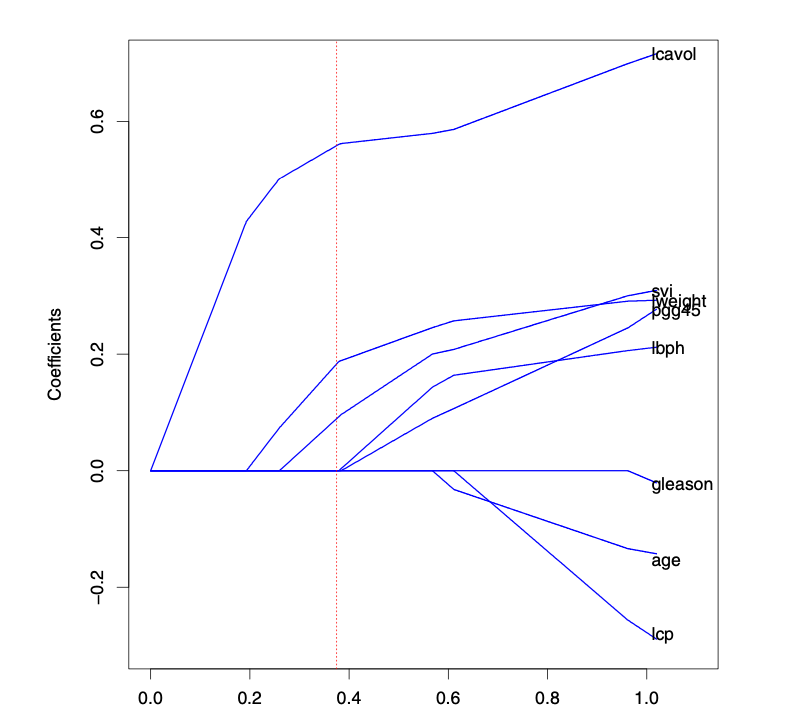
\includegraphics[width=4in]{HASTIE-LASSO.png}
(Here is an example of L1, also called LASSO, regularization from Hastie Elements of Statistical Learning Figure 3.10. 
High regularization is to the left.  Low regularization reproduces problem 1, high regularization eventually sets all
coefficients to zero.)

\item
SVD
Perform Singular Value Decomposition on all the features of the UCI Credit Default dataset.
Display scatter plots of PC1 vs PC2 for default and non-default classes.  
Label the axes with the fraction of the variance in PC1 and PC2.
Compute a table with the fraction of the variance in each of the first few principal components.

\item 
Perform L1-regularized logistic regression on the SVD-transformed features and plot the feature coefficients 
as a function of the logarithm of the regularization parameter. 
Find the optimum regularization parameter by minimizing error on the test set.  Does the optimum 
include more or fewer features than the standardized (but not coordinate-transformed) model?

\end{enumerate}
\end{document}


